\documentclass{article}
\usepackage{pgfplots}
\pgfplotsset{compat=1.18}

\begin{document}

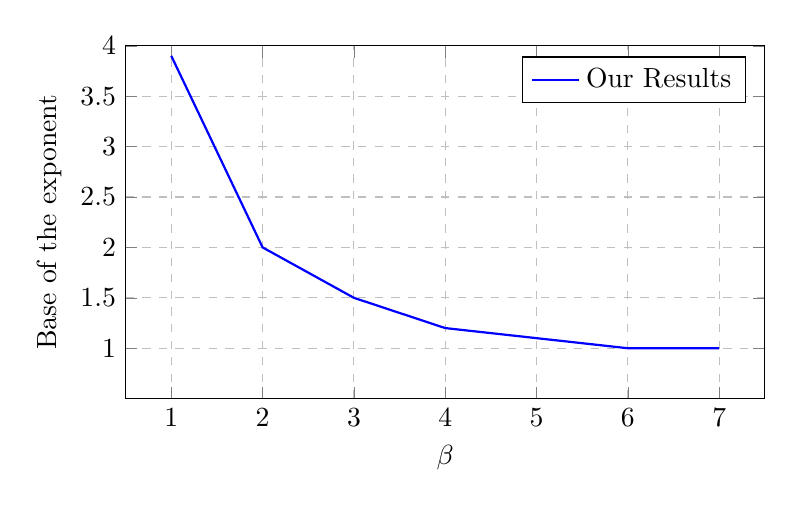
\begin{tikzpicture}
    \begin{axis}[
        xlabel={$\beta$},
        ylabel={Base of the exponent},
        grid=major,
        legend pos=north east,
        width=0.8\textwidth,
        height=0.5\textwidth,
        xmin=0.5, xmax=7.5,
        ymin=0.5, ymax=4,
        xtick={1,2,...,7},
        ytick={1,1.5,...,4},
        ymajorgrids=true,
        xmajorgrids=true,
        grid style=dashed,
    ]
        \addplot[blue, thick, mark=none] coordinates {
            (1, 3.9)
            (2, 2.0)
            (3, 1.5)
            (4, 1.2)
            (5, 1.1)
            (6, 1.0)
            (7, 1.0)
        };
        \legend{Our Results}
    \end{axis}
\end{tikzpicture}

A plot of the running time of our algorithm for \povd. The \(x\)-axis corresponds to the approximation ratio, while the \(y\)-axis corresponds to the base of the exponent in the running time. A point \((\beta, d)\) in the plot describes a running time of the form \(d^{k} \cdot n^{\Oh(1)}\) for a \(\beta\)-approximation.

\end{document}